%%%%%%%%%%%%%%%%%%%%%%%%%%%%%%%%%%%%%%%%%%%%%%%%%%%%%%%%%%%%%%%%
% Template for BI-ZUM final report
% Encoding: UTF8
% Version: 1.0 (2013-01-28)
% Author: Ing. Martin Šlapák
%%%%%%%%%%%%%%%%%%%%%%%%%%%%%%%%%%%%%%%%%%%%%%%%%%%%%%%%%%%%%%%%
\documentclass[a4paper,10pt,twocolumn]{article}
\usepackage{lmodern}
\usepackage[english]{babel}
\usepackage[T1]{fontenc}
\usepackage[utf8]{inputenc}
\usepackage{amsfonts}
\usepackage{mathtools}
\usepackage{graphicx}
\usepackage{listings}
\usepackage{url}
\lstset{basicstyle=\normalfont\small,breaklines=true,columns=flexible}
\usepackage{float}
\usepackage[top=0.5cm,bottom=2cm,left=1cm,right=1cm]{geometry}
%%%%%%%%%%%%%%%%%%%%%%%%%%%%%%%%%%%%%%%%%%%%%%%%%%%%%%%%%%%%%%%%
% Source: http://tex.stackexchange.com/questions/47175/scala-support-in-listings-package
% "define" Scala
\lstdefinelanguage{scala}{
  morekeywords={abstract,case,catch,class,def,%
    do,else,extends,false,final,finally,%
    for,if,implicit,import,match,mixin,%
    new,null,object,override,package,%
    private,protected,requires,return,sealed,%
    super,this,throw,trait,true,try,%
    type,val,var,while,with,yield},
  otherkeywords={=>,<-,<\%,<:,>:,\#,@},
  sensitive=true,
  morecomment=[l]{//},
  morecomment=[n]{/*}{*/},
  morestring=[b]",
  morestring=[b]',
  morestring=[b]"""
}
%%%%%%%%%%%%%%%%%%%%%%%%%%%%%%%%%%%%%%%%%%%%%%%%%%%%%%%%%%%%%%%%
%gobble gobbles page numbers so there are none
\pagenumbering{gobble}
\title{Different approaches to solving the 0-1 Knapsack problem}
\date{\today}
%%%%%%%%%%%%%%%%%%%%%%%%%%%%%%%%%%%%%%%%%%%%%%%%%%%%%%%%%%%%%%%%
% tady nastavte své jméno a email
\author{Grant Zvolský \\ zvolsgra@fit.cvut.cz}
%%%%%%%%%%%%%%%%%%%%%%%%%%%%%%%%%%%%%%%%%%%%%%%%%%%%%%%%%%%%%%%%
\begin{document}
\maketitle
%%%%%%%%%%%%%%%%%%%%%%%%%%%%%%%%%%%%%%%%%%%%%%%%%%%%%%%%%%%%%%%%
\begin{abstract}
This report summarizes the implementation of different approaches to solving the 0-1 Knapsack problem. A simple
heuristic as well as a naive solution were implemented, tested and evaluated. The implementation language is Scala.
\end{abstract}

%%%%%%%%%%%%%%%%%%%%%%%%%%%%%%%%%%%%%%%%%%%%%%%%%%%%%%%%%%%%%%%%
\section{Problem specification} % specifikaci úlohy (stručně, je možno použít odkaz na popis)
The Knapsack problem is an optimization problem. Let me quote Wikipedia for its definition.

\begin{quote}
The knapsack problem or rucksack problem is a problem in combinatorial optimization:
Given a set of items, each with a weight and a value, determine the number of each item
to include in a collection so that the total weight is less than or equal to a given limit
and the total value is as large as possible.\cite{wikiKnapsack}
\end{quote}

In this paper we look into a variation of the problem where each item can be included
at most once. This variation is known by the name 0-1 knapsack problem. In other words:

Let $M, n\in\mathbb{N}$ and $\forall i\in\{1, ..., n\}:v_i, m_i\in\mathbb{N}$.

Find $\{x_1, ..., x_n\}\in\{0, 1\}$
such that

\vspace{0.4em}
{\centering
$\sum_{i=1}^{n} x_i w_i \le M$ \quad and \quad $\sum_{i=1}^{n} x_i v_i = MAX$

}

\section{Breakdown of different approaches} % rozbor možných variant řešení
Solutions to the knapsack problem can be divided into these that guarantee finding the optimal solution, and these that
try to approximate it. I developed three solutions while working on this project. The first is an approximative solution
which uses a simple heuristic. The other two methods find the optimal solution by searching the whole state space.

\section{Solutions}
\subsection{Value/Weight Ratio Heuristic}
The following algorithm has the asymptotic computational complexity of the sorting algorithm it uses,
which is $\mathcal{O}(n\log{}n)$ in our case.
\begin{lstlisting}
Step 1: Sort the array of items by their value/weight ratio.
Step 2: Try adding items in this order. If an item is too large to fit, skip it.
\end{lstlisting}
That's all. The heuristic is very straightforward and yields surprisingly accurate results, see figure \ref{vwratioavgerr}.

\subsection{Naive Iteration}
The knapsack can be seen as a vector of booleans, where each boolean signifies the presence of absence of a particular
item. In a computer, an integer is also, technically, a vector of booleans. Therefore each knapsack configuration can be
seen as a numeric value, and iterating from $0$ to $2^n$ is analogous to iterating over all configurations. This naive
solution seems quite elegant, but there's a catch. Iterating over individual bits of each configuration in order to
calculate its weight and value has an asymptitic complexity of O(n). The overall asymptotic complexity of this approach
thus $\mathcal{O}(n\cdot2^n)$. Can we do better?

\subsection{Naive Recursion} \label{naiverec}
Another way to look at all the possible item combinations is a binary tree.
\begin{lstlisting}
1. The root represents an empty knapsack.
2. Right children at level i+1 include item i.
3. Left children at level i+1 do not include item i.
\end{lstlisting}
Traversing such tree makes it easy to keep track of the weight and value of given node. No significant computations are
required, which makes the worst case complexity the same as the number of nodes, $\mathcal{O}(2^n)$.

\section{Implementation} % popis kostry algoritmu (nikoliv výpis kódu!)
I chose Scala as the implementation language for its simplicity. See scaladoc comments in the code for implementation
details.

The project is structured into classes. Different algorithms are in separate files, e.g. NaiveIteration.scala. The
following code listing is my most effective naive solution, from the file NaiveRecursionSansConfigVars.scala. It
traverses the state space tree described in \ref{naiverec}.

\begin{lstlisting}[language=scala]
val items: Array[(Int, Int)] = ???
val capacity: Int = ???
var bestW, bestV = 0

def go(w: Int, v: Int, idx: Int): Unit = {
  if (w > capacity) return
  if (v > bestV) { bestV = v; bestW = bestW }
  if (idx == items.length) return
  go(w, v, idx + 1)
  go(w + items(idx)._1, v + items(idx)._2, idx + 1)
}
\end{lstlisting}

\section{Results} % naměřené výsledky v přehledné formě (nikoliv nepřehledná změť dat)
\vbox{
The first graph demonstrates the performance of the Naive Recursion Sans Config Vars -- a variation of the recursive
solution which doesn't keep track of exactly which items are inside the knapsack. It shows the relationship between
computation time and n, where n is the total number of items. As expected, it matches the $2^n$ reference curve.

\begin{figure}[H]
  \begin{center}
    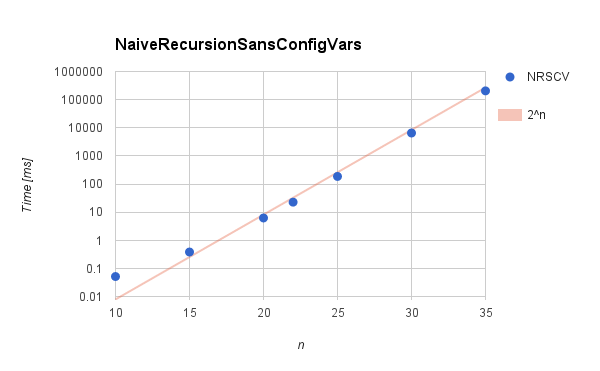
\includegraphics[width=10cm,height=6cm]{nrscv.png}
  \end{center}
  \caption{Naive Recursion}\label{fig1}
\end{figure}

\begin{figure}[H]
  \begin{center}
    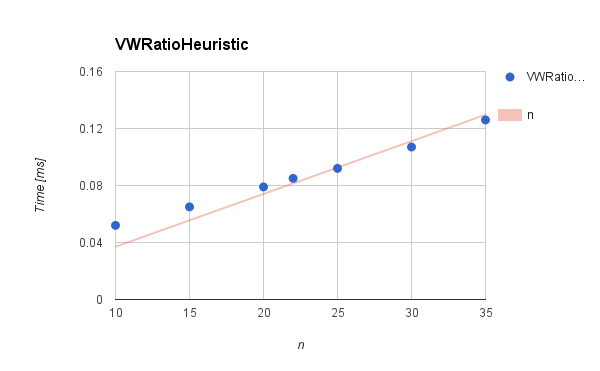
\includegraphics[width=10cm,height=6cm]{heuristic.png}
  \end{center}
  \caption{Value/Weight Ratio Heuristic}\label{fig1}
\end{figure}
}

The following tables show the average and maximum relative errors of the VWRatioHeuristic algorithm. The
following formula was used to calculate the relative error of a signle solution: \\

$\varepsilon = \frac{V(OPT)-V(APX)}{V(OPT)}$ \\

Where $V(OPT)$ is the value of the optimal solution and $V(APX)$ is the value of the optimal solution.

\begin{figure}[H]
    \begin{lstlisting}[basicstyle=\scriptsize]
    n     4      10      15      20     22      25      30     35    40
    avgE  1.94%  1.43%   .49%    .54%   .69%    .72%    .72%   .50%  .53%
    \end{lstlisting}
    \caption{Average error of the V/W ratio heuristic.}\label{vwratioavgerr}
\end{figure}

\begin{figure}[H]
    \begin{lstlisting}[basicstyle=\scriptsize]
    n      4      10     15     20     22     25      30     35     40
    maxE   24.7%  11.5%  8.54%  8.43%  7.23%  3.68%   5.51%  4.60%  2.34%
    \end{lstlisting}
    \caption{Maximal error of the V/W ratio heuristic.}\label{vwratiomaxerr}
\end{figure}

As we can see, the heuristic was fairly successful at finding near-optimal solutions and its precision increases with
the number of items.


\section{Conclusion} % závěr: interpretace výsledků a zdůvodnění jejich kvality
The Naive Iteration algorithm turned out to perform much worse than recursion. On the other hand, the recursive
algorithm and the heuristic performed to our expectations in regard to computational complexity.

The value/weight ratio heuristic yielded surprisingly good results, within 2\% of the optimal solutions. Other methods,
such as simulated evolution, may give even better approximations with little increase in time complexity.

\begin{thebibliography}{9}
    \bibitem{wikiKnapsack}
        Knapsack problem.
        In: \textit {Wikipedia} [online].
        [vid. 12.10.2016]. Available at:
        \url{https://en.wikipedia.org/wiki/Knapsack_problem}
\end{thebibliography}

\end{document}